\documentclass{article}

\usepackage{amsmath}
\usepackage{amsfonts}
\usepackage[utf8]{inputenc}
\usepackage{graphicx}
\usepackage{multicol}
\usepackage{multirow}
\usepackage{subcaption}
\usepackage{hyperref}
\hypersetup{
    colorlinks=true,
    linkcolor=blue,
    filecolor=magenta,      
    urlcolor=cyan,
}
\urlstyle{same}
\setlength{\parskip}{1em}
\graphicspath{ {./images/} }

\title{Sections and Chapters}
\author{Gubert Farnsworth}
\date{ }

\begin{document}
\maketitle
\tableofcontents

\newpage

% ==============================================================
% Introduction
% ==============================================================
\section{Introduction}

% ==============================================================
% GANS
% ==============================================================
\section{Background}
% ==============================================================


% ==============================================================
\subsection{Convolutional Neural Networks}
% ==============================================================
Convolutional Neural Networks, also known as ConvNets or CNNs, are the state-of-the-art neural networks for most computer vision tasks, such as image classification and object detection or face recognition.

Unlike regular feed-forward neural networks based on fully-connected layers of neurons, ConvNets are trained to learn relatively small filter kernels, that can extract valuable information from different areas of an image. Therefore, they reduce the amount of training parameters significantly and are able to train also on large images.

% ==============================================================
\subsubsection{Convolution}
% ==============================================================
The cornerstone of ConvNets are the convolutions, represented in Figure \ref{fig:conv}. Convolutions are based on small filters, which run through the image and sum the multiplications of each input value with the corresponding filter value. Each filter must have the same amount of channels as the input, the width and height are optional. 

\begin{figure}[h]
\centering
{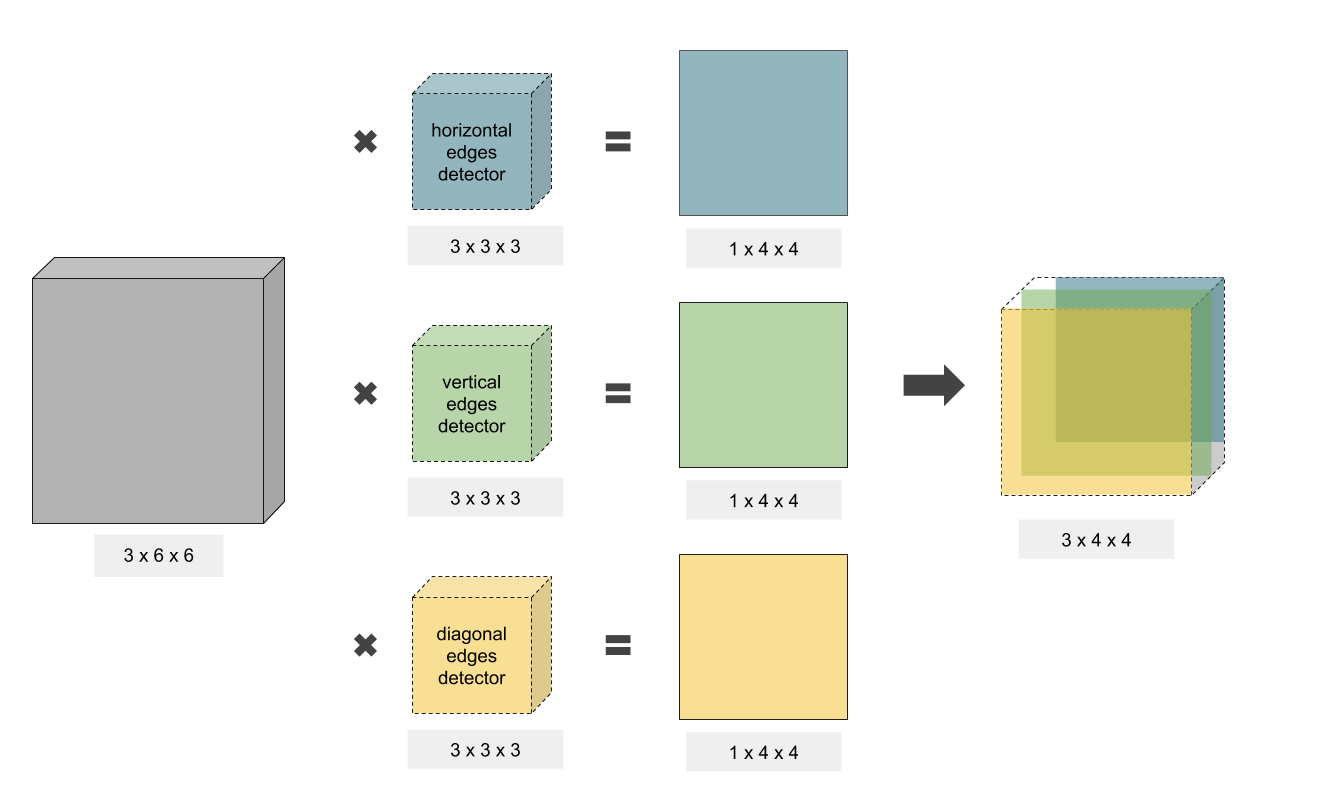
\includegraphics[width=\linewidth]{GAN/convolutions}}
\caption{\label{fig:conv} \textbf{Convolution.} The input image is convolved with 3 filters, each one detecting a different low-level feature. The final output is the output of each convolution stack in the channel dimension.}
\end{figure}


\subsubsection{Convolutional Layers}
In the first layers of a network, each filter usually extracts some low-level feature, such as horizontal or vertical edges. The output of the convolution, are the outputs of each filter stacked in the channel dimension. As the convolutions get deeper into the network, they start to combine these low-level features, to higher level features, such as an eye or a mouth.





% ==============================================================
\subsection{Generative Adversarial Networks}
% ==============================================================

Introduced in 2014 \cite{goodfellow_generative_2014}, generative adversarial  networks, so-called GANs, have been the focus of countless research papers and creative implementations. GANs have learned how to generate an image of a cat from a simple drawing \cite{hesse_image--image_nodate}, create new artworks \cite{rkjones4_gangogh:_2018}, generate high-resolution celebrity faces \cite{karras_progressive_2017}, colorize grayscale images and much more.

In order to generate new samples, two neural networks are trained to compete against each other. A common analogy can be found in coin forgery: while a fraud investigator is trying to detect real coins from fraudulent ones, the coin forger is trying to improve the falsification, so that the investigator is unable to tell the difference.

In computational world, the investigator is a neural network called \textit{Discriminator} competing with the forger network called \textit{Generator}. The discriminator is trained to classify samples from the original dataset as "real", and samples generated by the generator as "fake". The generator is trained to fool the discriminator, so that he cannot correctly classify the generated samples as fake.

\begin{figure}[h]
\centering
\subcaptionbox{Original MNIST}
{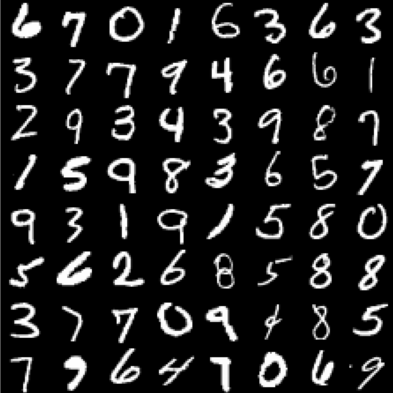
\includegraphics[height=4cm]{GAN/mnist_orig}}\hspace{1cm}
\subcaptionbox{Generated MNIST}
{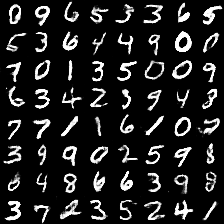
\includegraphics[height=4cm]{GAN/mnist_dcgan}}
\caption{\label{fig:mnist} \textbf{MNIST Example.}
(a) Example of data points in the original MNIST dataset \cite{lecun_mnist_nodate}. (b) Samples generated with a Deep Convolutional GAN \cite{kim_dcgan-tensorflow:_2018}.}
\end{figure}

Figure \ref{fig:mnist} shows example data points of the hand-written digits dataset MNIST \cite{lecun_mnist_nodate}, along with samples generated with a deep convolutional GAN \cite{kim_dcgan-tensorflow:_2018} - the samples from the original and generated distributions are almost indistinguishable.


% ==============================================================
\subsubsection{Architecture}
% ==============================================================

Figure \ref{fig:gan} describes a typical GAN architecture. The discriminator is a common Convolutional Neural Network \cite{lecun_convolutional_1995}, which takes an image as input and is trained to find filters that extract necessary information in order to classify the image. The output is a 1-dimensional vector - or in case of GANs, a scalar value, classifying the image as real or fake. 

The generator's architecture is similar, however it uses a transposed convolution, the so-called "deconvolution", to produce a 2 or 3-dimensional output from a 1-dimensional input vector. The generator input vector is sampled randomly.

\begin{figure}[h]
\centering
{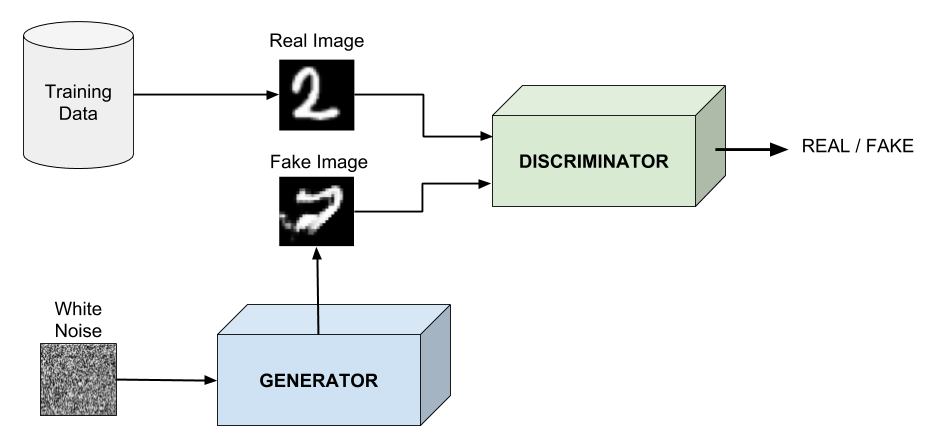
\includegraphics[width=\linewidth]{GAN/gan_model}}
\caption{\label{fig:gan} \textbf{GAN model.} The generator network produces fake images, which the discriminator network tries to distinguish from the real samples coming from the dataset.}
\end{figure}

The classification output of the discriminator is back-propagated  through the discriminator, as well as the generator network, in order to adjust the networks' weights to improve the training objective.

% ==============================================================
\subsubsection{Training Objective} \label{sec:GAN_training}
% ==============================================================

Given input data with distribution $p(x)$, the generator $G$ is a neural network, that maps random input noise $z$ to the input space, as $G(z, \theta_{g})$, learning the model distribution $\hat{p}(x)$. The discriminator $D$ is a second neural network $D(x, \theta_{d})$ with a single scalar output, classifying the input as real, sampled from $p(x)$, or as fake, sampled from the model distribution $\hat{p}(x)$. 

The training objective of the discriminator is to maximize the probability of assigning the correct label, while the objective of the generator is to minimize this probability. The loss function of the GAN can be described as the minimax objective,

\begin{equation}
\underset{G}{\mathrm{min}} \ \underset{D}{\mathrm{max}} \ V(D,G) = \mathbb{E}_{x \sim p_{data}(x)}[\log D(x)] + \mathbb{E}_{z \sim p_{z}(z)}[\log 1 - D(G(z))].
\label{eq:minimax}
\end{equation}

In order to prevent vanish gradients, as a result of the discriminator saturating by confidently classifying the samples before the generator's update, \cite{goodfellow_generative_2014} suggests $G$ to be trained to maximize $\mathbb{E}_{z \sim p_{z}(z)}[\log D(G(z))]$ instead.

The parameters of the discriminator and generator, $\theta_{d}$ and $\theta_{g}$, are updated using backpropagation algorithm, computing the gradients of the loss function in respect to each network's parameters. 


% ==============================================================
\subsubsection{Training Difficulties}
In theory, the minimax game described in equation \ref{eq:minimax} is played until generator has perfectly modeled the distribution $p(x)$, so that discriminator classifies the authenticity of the samples at random. 

In reality, finding the right balance between the two networks is one of the difficulties when training a GAN. If discriminator gets too good at determining which samples are fake, then generator has no chance to learn the distribution. On the other hand, if generator is updated too much, it can collapse too many values of $z$ to the same value of $x$ to have enough diversity to model the distribution.

% ==============================================================
% Deep Convolutional GANs
% ==============================================================
\subsubsection{Deep Convolutional GANs}

\begin{figure}[h]
\centering
{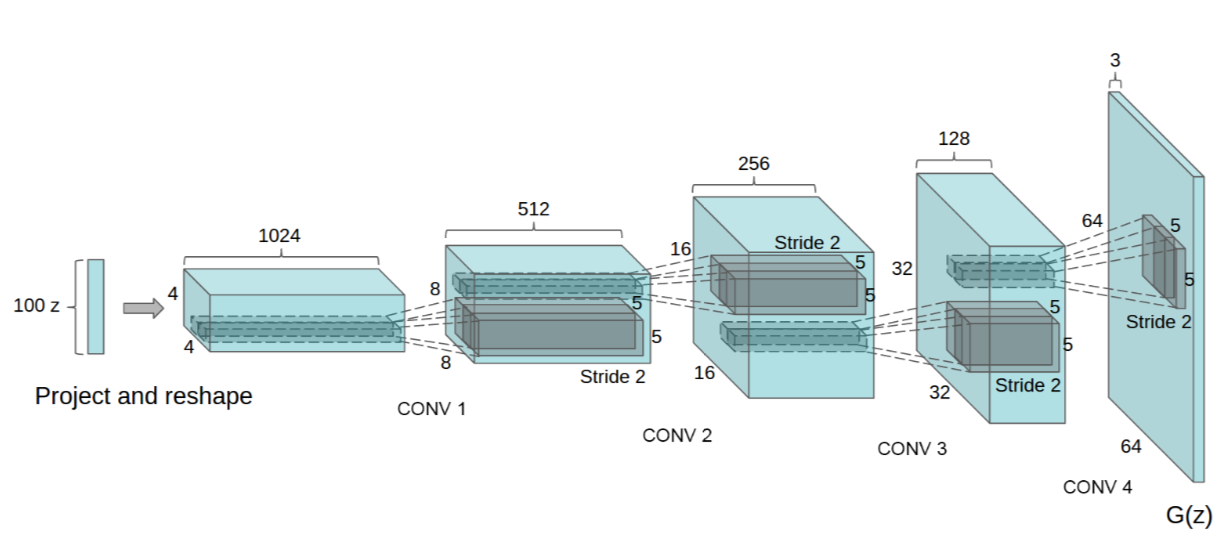
\includegraphics[width=\linewidth]{GAN/dcgan_generator}}
\caption{\label{fig:dcgan} \textbf{DCGAN Generator.} An example architecture of a DCGAN generator $G(z)$. The random input noise $z$ is mapped to a 64x64 image with 3 color channels via fractionally-strided convolution layers. Figure reprinted from \cite{radford_unsupervised_2015}.}
\end{figure}

Many GAN implementations base their network architecture on Deep Convolutional GANs, described by \cite{radford_unsupervised_2015}. The authors introduced architectural guidelines for convolutional networks used in GANs, that stabilize the training and result in more realistic outputs.

After experimenting with CNN architectures commonly used in computer vision tasks, Radford et al. have found that this set of architecture modifications has a positive effect on the stability and convergence speed of the models:
\begin{itemize}
\item \textbf{All Convolutional Net}: A common practice in convolutional neural networks are \textit{Pooling Layers}, which reduce the number of parameters by filtering the convolution outputs, taking maximum or average of a given region. However, the authors have found that using an All Convolutional Network \cite{springenberg_striving_2014}, which replaces all pooling layers with a strided convolution, leads to more stable results.
\item \textbf{Fully-Connected Layers}: The authors argue, that avoiding fully-connected layers deeper in the network stabilizes the network. Removing all fully-connected layers stabilizes the network, however it slows down the convergence. Therefore fully-connected layers are kept in the discriminator output layer and generator input layer. 
\item \textbf{Batch Normalization}: Batch Normalization \cite{ioffe_batch_2015} has been introduced in common image-classification to make models more robust to parameter initialization and speed up training. The DCGAN paper shows that including a batch-norm layer in all GAN layers (except discriminator output and generator input), helps generators start learning and produce diverse outputs.
\item \textbf{Activation Functions}: As opposed to maxout activation suggested by the original GAN paper \cite{goodfellow_generative_2014}, GANs seem to benefit from \textit{Leaky ReLU} activation function in discriminator, and \textit{ReLU} activation function for generator, except last \textit{tanh} layer. 
\end{itemize}



% ==============================================================
% Conditional GANs
% ==============================================================
\subsubsection{Conditional GANs}
In order to influence the output of a GAN, \cite{mirza_conditional_2014} introduced the Conditional Generative Adversarial Networks. By conditioning both the discriminator and the generator on additional information, the generator learns to output realistic samples given a condition. 

Considering the previous example of MNIST hand-written digits synthesis, one can condition the networks using the digits as class labels, and control the network to generate an image of a specific digit. There have also been experiments with text-to-image translation \cite{reed_generative_2016}, where the network is conditioned on a text description of an image, and various image-to-image translations such as \cite{yoo_pixel-level_2016}, \cite{yoo_pixel-level_2016}, \cite{pathak_context_2016}.

 The training objective of conditional GAN is following:
\begin{equation}
\underset{G}{\mathrm{min}} \ \underset{D}{\mathrm{max}} \ V(D,G) = \mathbb{E}_{x \sim p_{data}(x)}[\log D(x|c)] + \mathbb{E}_{z \sim p_{z}(z)}[\log 1 - D(G(z|c))].
\label{eq:cgan}
\end{equation}

The conditioning information $c$, such as a class label, text, or another image, is fed to both discriminator $D$ and generator $G$ as additional input layers. For example, conditioning a MNIST image on the label 7, 



% ==============================================================
\section{Analysis}
% ==============================================================

% ==============================================================
% DATA
% ==============================================================
\subsection{Data}
As in most machine learning algorithms applied to visual tasks, the quantity and quality of training data is essential to produce high-quality results. It is also common, that data collection and data cleaning make up a significant part of a machine learning project.

In case of fashion images, there are several open-source datasets published online. However, after careful evaluation I have not found them sufficient for the type of tasks I wanted to achieve. Therefore I have created an application that can scrape an online fashion store to download images of fashion products and their description in a computer-readable format.

% ==============================================================
\subsubsection {Requirements}
% ==============================================================

In order to generate high-quality outputs using GANs, the collected dataset should fulfill the following requirements as much as possible:
\begin{enumerate}
\item The fashion products should be photographed on a white background. 
\item There should be a machine-readable description of each product, such as color, shape, category, etc. 
\item The images should be in a sufficient resolution.
\item There should be a sufficient amount of images of various items.

\end{enumerate}
I have defined these requirements on based on my previous experience with generative algorithms. It is generally easier for the algorithm to focus on the important attributes of the images, if there are no distractions in terms of different model poses, backgrounds, etc. And since the main point of the project is to modify different attributes of the products, the images need to be labeled.

% ==============================================================
\subsubsection {Existing Fashion Datasets}
% ==============================================================

The existing datasets that consist or include images of fashion items do not fulfill the criteria of the dataset for the application. 

\paragraph{DeepFashion}
The Deep Fashion Set \cite{the_chinese_university_of_hong_kong_deepfashion_nodate} includes a very extensive Attribute Prediction collection, with more than 200.000 images of clothing images, labeled with 1000 attributes. However, this dataset does not fulfill the first requirement, with its clothing items photographed on people in various poses and backgrounds. This type of variation might be too complex for the algorithms and can lead to unsatisfactory results.

\paragraph{Fotolia}
Another available option, that has been provided by Prof. Dr. Barthel, is the Fotolia image dataset, which can be explored on the picsbuffet website \cite{noauthor_picsbuffet_nodate}.

To test the dataset, I have chosen all images with keywords "dress" and "isolated" and compared them to a template image, based on L1 distance between their 64-dimensional feature vectors. Figure \ref{fig:fotolia} shows the results of this search. The 64-dimensional feature vectors were calculated via Akiwi API \cite{sonnenberg_akiwi_nodate}.

\begin{figure}[h]
\centering
\subcaptionbox{Template Image}{\fbox{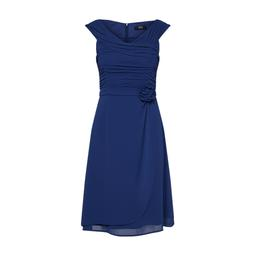
\includegraphics[height=3cm]{dress_template}}}\hspace{1cm}
\subcaptionbox{Fotolia Images}{\fbox{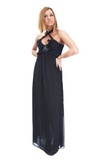
\includegraphics[height=3cm]{fotolia_ex1}}
\fbox{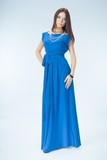
\includegraphics[height=3cm]{fotolia_ex2}}
\fbox{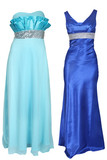
\includegraphics[height=3cm]{fotolia_ex3}}}
\caption{\label{fig:fotolia} Fotolia images with keywords "dress" and "isolated" with closest feature vector distance from the template image.}
\end{figure}


Additionally to an undesired low resolution of the returned images - around 100 x 160 pixels - the results also have too much variety, such as different model poses, different zoom levels and backgrounds. The description of the images did not include many useful attributes, with most pictures being labeled with words such as: "beauty", "young", "person", and lacking information about colors, shapes and pattern.

% ==============================================================
\subsubsection{Scraped Dataset}
% ==============================================================
Based on the evaluation of existing fashion datasets, I have identified a need for creating a new dataset specifically for the requirements of the application. I evaluated several fashion e-shops, from which images of the products and their descriptions could be downloaded. 

I chose 3 websites, based on the structure and amount of information they provide: \href{https://www.zalando.de/damen-home/}{zalando.de}, \href{https://www.aboutyou.de/}{aboutyou.de} and \href{https://www.fashionid.de/damen/}{fashionid.de}. Each of them provides several thousand fashion products for women and men, with a photograph of the item on a white background and some basic description such as color, pattern, shape, length etc. For simplicity, I have limited the dataset to women's clothes, excluding products like accessories and shoes.

The fashion scraper is python project, that scrapes images and data from all the mentioned websites and saves them locally for further processing, such as image processing, data cleaning, joining and translating. This project was part of my Independent Coursework and the documentation of the project can be found in Attachments, or on \href{https://github.com/sonynka/fashion_scraper}{github.com/sonynka/fashion\_scraper}.

\begin{figure}[h]
\centering
{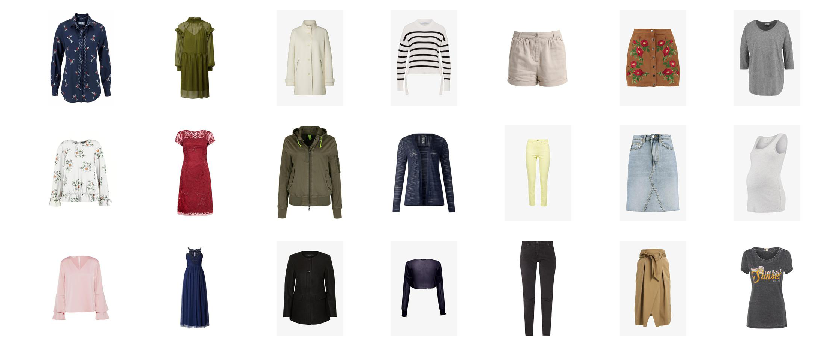
\includegraphics[width=\linewidth]{dataset_examples/img_grid2}}
\caption{\label{fig:dataset} \textbf{Examples of images in the final dataset.} Each column contains images from different category as follows: blouses, dresses, jackets, knitwear, pants, skirts, tops.}
\end{figure}

The scraped dataset consists of 92.200 images of size 256x256 pixels in JPEG format. The images are split into folders by categories and the whole dataset is described in a CSV file, which includes the following information:
\begin{itemize}
\item \textbf{id}: ID of the product as defined by the website (SKU)
\item \textbf{img\_path}: relative local file path to the saved product image
\item \textbf{img\_url}: URL to the product image file hosted on the seller website
\item \textbf{model\_img\_urls}: URLs to the images of the product worn by models
\item \textbf{product\_url}: if given, the URL to the product listing on the website
\item \textbf{brand}: product brand as displayed on the website
\item \textbf{name}: product name as displayed on the website
\item \textbf{attributes}: list of product attributes listed on the website in German, such as shape, length, material, size etc.
\end{itemize}

In addition to the website data, there are columns that contain processed and translated data. Below is the list of the column names and the values they can take.
\begin{itemize}
\item \textbf{category}: blouses, dresses, jackets, knitwear, pants, skirts, tops
\item \textbf{color}: beige, black, blue, gray, green, pink, red, white, yellow
\item \textbf{length}: 3-4, knee, long, normal, short or no value
\item \textbf{sleeve\_length}: half, long, short, sleeveless or no value
\item \textbf{fit}: loose, normal, tight or no value
\item \textbf{pattern}: floral, lace, polkadots, print, stripes, unicolors or no value
\item \textbf{neckline}: back, deep, lines, round, v, wide or no value
\end{itemize}

\marginpar{A table with all attributes and num of images will be in attachments}
There is also a CSV file that contains a list of image file paths and binary classification of the list of values mentioned in the above list.

% ==============================================================
\subsection{Image-To-Image Translation}
% ==============================================================

Lot of papers and open-source repositories have been published since the appearance of the original GAN paper. I have reviewed and tested several of them, in order to find architectures and code applicable to the problem of generating and modifying fashion images. 

Based on various characteristics, compared in Table \ref{tab:gan_comp}, I have evaluated  5 networks: pix2pix \cite{isola_image--image_2016}, CycleGAN \cite{zhu_unpaired_2017}, StarGAN \cite{choi_stargan:_2017}, MUNIT \cite{huang_multimodal_2018} and FaderNetworks \cite{lample_fader_2017}. I have compared the following attributes for each of the mentioned networks:
\begin{itemize}
\item Supervised/Unsupervised learning: Describes if the network needs a dataset consisting of paired images, such as the same skirt in a short and log version.
\item Multi-Domain: Describes if the network is able to train only one model for different domain modifications, or if each domain requieres its own trained generator.
\item Multi-Modal: Describes if the network is able to generate different versions from the same input.
\item Latent representation: Describes if the network trains directly in pixel-space or uses latent representation of the data, usually content and style of the images.
\end{itemize}

\begin{table}
\centering
\begin{tabular}{l*{5}{c}}
Network Characteristics & pix2pix &	CycleGAN & StarGAN	& MUNIT	& FaderNetworks \\
\hline
Supervised Training		& Yes & No & No & No & No \\
Multi-Domain  			& No  & No & Yes & No & No \\
Multi-Modal				& No & No & No & Yes & No \\
Latent Representations	& No & No & No & Yes & Yes \\
\end{tabular}
\caption{\label{tab:gan_comp}\textbf{Comparison of existing GAN models based on their characteristics.} Supervised training means that the dataset consists of image pairs, e.g: a dress and a person wearing the dress. Multi-Domain networks are able to train one model to change multiple attributes. Multi-Modal networks are able to generate more than one possible output. Networks with latent representations try to model the training data in a latent space, as opposed to pixel space.}
\end{table}

% ==============================================================
\subsubsection{Pix2Pix}
% ==============================================================
The so-called pix2pix networks were first introduced by Isola et al. \cite{isola_image--image_2016} as a framework for image-to-image translations using conditional neural networks. Some of the applications of pix2pix include mapping day photographs to night, sketches of shoes to realistic shoe images or colorizing black-and-white photos.

Pix2Pix uses the concept of conditional GANs \cite{mirza_conditional_2014}, where the network's output can be influenced by providing a class label $c$. The class label is fed to both the generator $G(z|c)$ and discriminator $D(x|c)$ as an additional input layer.

In case of pix2pix, the network is trained to translate images from an input domain to a target domain, requiring a dataset of paired images $(x_{input}, x_{target})$, such as a photograph of a street during the day and a corresponding night photograph of the same street. In addition to the generator mapping the random noise $z$ to target domain $\hat{x}_{target}$, it is also conditioned on the input image $x_{input}$, such as $G: (x_{input}, z) \rightarrow \hat{x}_{target}$.

The adversarial objective, which $G$ is trained to minimize and $D$ is trained to maximize, can be expressed as following:

\begin{equation}
\mathcal{L}_{adv}(D,G) = \mathbb{E}_{x_{in},x_{trg}}[\log D(x_{in},x_{trg})] + \mathbb{E}_{x_{in},z}[\log 1 - D(x_{in}, G(x_{in},z))]
\label{eq:pix2pix_minimax_cond}
\end{equation}

Based on the results of previous conditional GAN approaches \cite{pathak_context_2016}, Isola et. al \cite{isola_image--image_2016} have also shown, that enforcing the generated output to be closer to the ground truth target by adding a second objective reduces artifacts in the results. They therefore suggest to use the L1 distance as reconstruction loss function for the generator to optimize.

\begin{equation}
\mathcal{L}_{rec}(G) = \mathbb{E}_{x_{in},x_{trg},z}[||x_{trg}-G(x_{in},z)||_{1}]
\label{eq:pix2pix_loss_rec}
\end{equation}


The final objective of the generator is:
\begin{equation}
G^{*} = arg \ \underset{G}{\mathrm{min}} \ \underset{D}{\mathrm{max}} \ \mathcal{L}_{adv}(D,G) + \lambda \mathcal{L}_{rec}(G)
\end{equation}
where $\lambda$ controls the relative importance of the two loss functions.


% ==============================================================
% CycleGAN
% ==============================================================
\subsubsection{CycleGAN}
CycleGANs \cite{zhu_unpaired_2017} also solve the image-to-image translation problem, but unlike pix2pix, they do not require a paired image set for the image domains. The unsupervised setting is preferred in most translation tasks, as obtaining image pairs of two domains can be difficult or even impossible, for example when translating faces of women to faces of men, or artworks of Monet to realistic photographs. The assumption of this approach, is that both image domains share certain underlying visual similarities.

\begin{figure}[t]
\centering
\subcaptionbox{CycleGAN Model}
{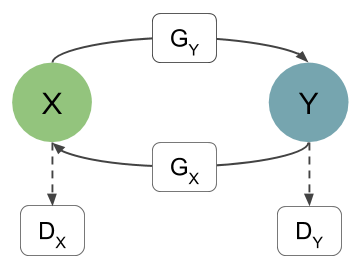
\includegraphics[height=4cm]{CycleGAN_graph}}\hspace{1cm}
\subcaptionbox{Cycle Consistency Loss}
{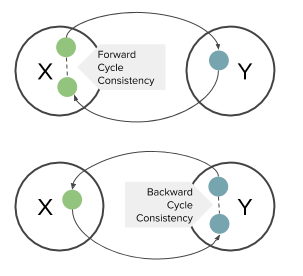
\includegraphics[height=4cm]{CycleGAN_graph2}}
\caption{\label{fig:cyclegan} (a) The CycleGAN model consists of two mappings, $G_{X}$ and $G_{Y}$ and corresponding discriminators $D_{X}$ and $D_{Y}$. (b) Cycle Consistency Loss measures the L1 distance between a real sample from one image domain and its encoded-decoded version. Figure adapted from \cite{zhu_unpaired_2017}.}
\end{figure}

The model consists of two generators, $G_{X}$ and $G_{Y}$, which learn mapping from image domain $X$ to image domain $Y$, $G_{Y}: X \rightarrow Y$, and vice versa. Each of the image domains has its own discriminator, $D_{X}$ and $D_{Y}$, that check if the given image comes from the real distribution of the domain or is translated from the opposite domain.

\begin{equation}
\mathcal{L}_{adv}(D_{X},G_{X}) = \mathbb{E}_{x}[\log D_{X}(x)] + \mathbb{E}_{y}[\log 1 - D_{X}(G_{X}(y))]
\label{eq:cyclegan_adv}
\end{equation}

Additionally to the adversarial loss, CycleGAN also implements a so-called \textit{Cycle Consistency Loss}, which enforces that an image encoded from one domain to another, can also be brought back to the original domain. The \textit{forward cycle consistency} defines that the  an image $x$ from domain $X$ and its encoded-decoded version should be approximately the same: $G_{X}(G_{Y}(x)) \approx x$. The \textit{backward cycle consistency} defines the same for an image from domain $Y$.

\begin{equation}
\mathcal{L}_{cyc}(G_{X},G_{Y}) = \mathbb{E}_{x}[||G_{X}(G_{Y}(x)) - x||_{1}] + \mathbb{E}_{y}[||G_{Y}(G_{X}(y)) - y||_{1}]
\label{eq:cyclegan_cycle}
\end{equation}

The authors argue, that by enforcing this encoder-decoder logic, the generators learn not to contradict each other. The final objective is:

\begin{equation}
\begin{split}
G^{*}_{X}, G^{*}_{Y} = arg \ \underset{G_{X}, G_{Y}}{\mathrm{min}} \ \underset{D_{X}, D_{Y}}{\mathrm{max}} \ \mathcal{L}_{adv}(D_{X},G_{Y}) \ +  \mathcal{L}_{adv}(D_{Y}, G_{X}) \\ + \ \lambda \mathcal{L}_{cyc}(G_{X}, G_{Y})
\end{split}
\end{equation}

% ==============================================================
% StarGAN
% ==============================================================
\subsubsection{StarGAN}
In case of Pix2Pix and CycleGAN, one of the disadvantages is the missing possibility multi-domain training. In other words, if there are more than 2 domains to translate between each other, one must train a new model for each domain pair. This can be time and computationally intensive.

StarGAN \cite{choi_stargan:_2017} is unique among the tested models, as it is able to train one single generator that maps input to multiple domains, as shown in Figure \ref{fig:stargan_topo}. Using the conditional GAN model, the generator is conditioned on a randomly chosen target domain each iteration, so that it can learn mapping for all given domains. 

Given an image $x$ and a target domain label $c_{trg}$, generator $G$ tries to minimize the adversarial loss objective, to generate real-looking images conditioned on the target domain, while the discriminator classifying the source of the image, $D_{src}$, tries to maximize it.

\begin{equation}
\mathcal{L}_{adv} = \mathbb{E}_{x}[\log D_{src}(x)] + \mathbb{E}_{x, c_{trg}}[\log 1 - D_{src}(G(x, c_{trg}))]
\label{eq:stargan_adv}
\end{equation}


Instead of feeding the target domain class $c$ to the discriminator, as in common conditional networks, StarGAN uses an auxiliary classifier GAN, AC-GAN \cite{odena_conditional_2016}. It forces the discriminator to output both the probability distribution over the sources of the input, and the probability of the target domain labels, $D: x \rightarrow {D_{src}(x), D_{cls}(x)}$. This improves the network's stability and performance, as it forces the discriminator to perform and additional task.

\begin{figure}[t]
\centering
\subcaptionbox{Cross-Domain Models}
{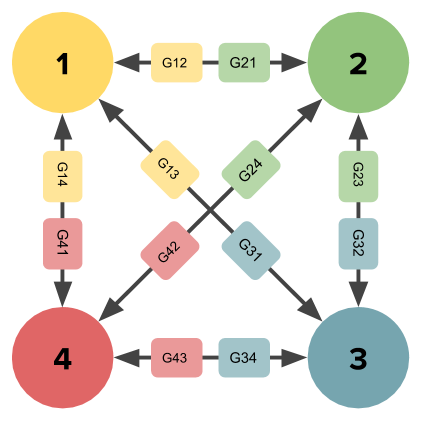
\includegraphics[height=4cm]{StarGAN_graph}}\hspace{1cm}
\subcaptionbox{StarGAN Model}
{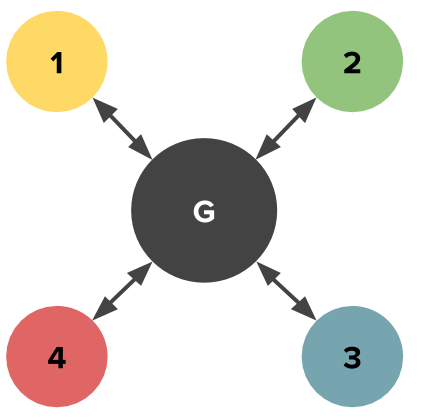
\includegraphics[height=4cm]{StarGAN_graph2}}
\caption{\label{fig:stargan_topo} \textbf{Comparison of cross-domain models and StarGAN model.} While cross-domain models need one generator per each domain pair, StarGAN only trains one generator for multiple domains. Figure adapted from \cite{choi_stargan:_2017}.}
\end{figure}

This modification to the discriminator introduces the \textit{Domain Classification Loss} with two objectives, optimizing $D$ and $G$ respectively. Given training data with an image $x$ and its original domain $c_{in}$, $D$ learns to classify the domain label correctly by minimizing the following objective:
\begin{equation}
\mathcal{L}^{r}_{cls} = \mathbb{E}_{x,c_{in}}[-\log D_{cls}(c_{in}|x)].
\label{eq:stargan_clsr}
\end{equation}

The generator objective is to generate images, that fool the auxiliary classifier and are classified as the target domain $c_{trg}$:
\begin{equation}
\mathcal{L}^{f}_{cls} = \mathbb{E}_{x,c_{trg}}[-\log D_{cls}(c_{trg}|G(x, c_{trg}))].
\label{eq:stargan_clsf}
\end{equation}

StarGAN \cite{choi_stargan:_2017} also uses the \textit{Cycle Consistency Loss} \cite{zhu_unpaired_2017}, in order to generate images that preserve the underlying content of the original image, and only change the domain-related attributes:
\begin{equation}
\mathcal{L}_{cyc} = \mathbb{E}_{x,c_{in},c_{trg}}[||x - G(G(x,c_{trg}), c_{in})||_{1}].
\label{eq:stargan_cyc}
\end{equation}


The full training objective for $D$ and $G$ respectively is:

\begin{equation}
\mathcal{L}_{D} = -\mathcal{L}_{adv} + \lambda_{cls} \mathcal{L}^{r}_{cls},
\label{eq:stargan_D}
\end{equation}
\begin{equation}
\mathcal{L}_{G} = \mathcal{L}_{adv} + \lambda_{cls} \mathcal{L}^{f}_{cls} + \lambda_{cyc} \mathcal{L}_{cyc},
\label{eq:stargan_G}
\end{equation}

where $\lambda_{cls}$ and $\lambda_{cyc}$ control the relative importance of the two loss functions against the adversarial loss.

% ==============================================================
% MUNIT
% ==============================================================
\subsubsection{MUNIT}
All of the introduced models approach the image translation problem as one-to-one mapping. However, many of the image domain translation tasks are in fact multi-modal, meaning one single input can have multiple different outputs. The MUNIT network \cite{huang_multimodal_2018} introduces an unsupervised multi-modal method, which is able to capture the diversity of the output.

Instead of using translation in pixel space, the model tries to model the translation in a latent space. Based on the \textit{partially shared latent space assumption}, a content latent code $c \in \mathcal{C}$ and a style latent code $s_{i} \in \mathcal{S}_{i}$ are separated, assuming that the two image domains share a common content space but each has an individual style space. 

For each domain, there is an auto-encoder, which consists of a generator $G$ and two encoders: content encoder $E^c$, and style encoder $E^s$. Given an image $x \in X$, it is encoded into a content and latent code, $E^c_x(x)$ and $E^s_x(x)$. To translate the image $x \in X$ to domain $Y$, its content code $c_{x}$ is extracted using the content encoder $E^c_x$, and it is combined with a random style code $s_{y}$, $G_y(c_x, s_y)$.


\textbf{Reconstruction Loss.}
The reconstruction loss is similar to the cycle consistency loss \cite{zhu_unpaired_2017}, enforcing the reconstruction between an image and its latent representation in both directions. $\mathcal{L}^{x}_{rec}$ encourages 
\begin{equation}
\mathcal{L}^{x}_{rec} = \mathbb{E}_{x}[||x - G_{x}(E^{c}_{x}(x), E^{s}_{x}(x))||_{1}]
\end{equation}
\begin{equation}
\mathcal{L}^{c_{x}}_{rec} = \mathbb{E}_{c_{x}, s_{y}}[||c_{x} - E^{c}_{y}(G_{y}(c_{x},s_{y}))||_{1}]
\end{equation}
\begin{equation}
\mathcal{L}^{s_{y}}_{rec} = \mathbb{E}_{c_{x}, s_{y}}[||s_{y} - E^{s}_{y}(G_{y}(c_{x},s_{y}))||_{1}]
\end{equation}


\textbf{Adversarial Loss.}



While the style code is assumed to have a global and simple effect and is therefore sufficiently represented by a low-dimensional vector, the content is assumed to be a high-dimensional vector describing the complex spatial structure of the data.


% ==============================================================
\section{Other}
% ==============================================================

\subsection{Model Images}
For some of the tasks of this project also images of people modeling the products were required.  However, each product, has multiple images of a model wearing it, and for the purposes of this project, I had to use clustering methods to filter out only images where the models are facing the front and photographed full-bodied.

\subsubsection{Clustering}
The supervised algorithms require a paired image set - in the case of generating model image from product image, it was neccessary to obtain images showing a person modelling the product. This could be obtained from the scraped websites, however each product usually has multiple model images - unordered, usually front-facing, back-facing, detail and cut. I have applied the K-Means clustering algorithm in order to separate these types of images, and for each product, find the front-facing model image.


\section{Products to Models}
One of the tasks of the framework is to generate a realistic image of a model wearing a product, given an image of the product. The motivation is to expand the amount of similar images found - as some products might not have a photograph without a model available at all.

I acquired the dataset for this task by downloading all model images for each product, as listed in the scraped data file. However, each product usually has multiple images with variety of model poses and detail; usually unordered and with no pattern that would indicate which image displays what pose. Therefore I have applied the K-means clustering algorithm to try to cluster these image by the model pose and for each product, select the image where the model is photographed front-facing and full-bodied.

\subsection{Clustering}



\newpage
\bibliographystyle{alphadin}
\bibliography{zotero}
\end{document}
